\section{Durchführung}
%
\subsection{Verstärkerschaltung mit einem Transistor in Emitterschaltung}
%
\subsubsection*{Dimensionierung}
%
Die berechnete Dimensionierung laut Tabelle \ref{tab:DimensionierungEmitterschaltung} wurden mit dem Versuchsbetreuer besprochen, abgeglichen und können verwendet werden.
%
\subsubsection*{Aufbau}
%
Wir bauen die Schaltung eines Transistors in Emitterschaltung mit Stromgegenkopplung auf wie in Abbildung \ref{fig:EmitterschaltungStromgegenkopplung} zu sehen.
Die fertige Schaltung ist in Abbildung \ref{fig:FotoTransistorschaltungen} dargestellt.
%
\par
%
\minipage{\linewidth}
    \begin{center}
        \captionsetup{type=figure}
        \begin{adjustbox}{max width=\linewidth, keepaspectratio}
            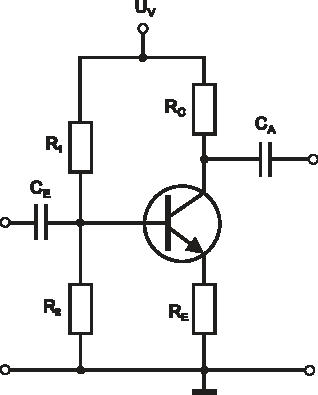
\includegraphics[]{pdf/EmitterschaltungStromgegenkopplung}
        \end{adjustbox}
        \captionof{figure}{Transistor in Emitterschaltung mit Stromgegenkopplung (Quelle \cite{Anleitung})}
        \label{fig:EmitterschaltungStromgegenkopplung}
    \end{center}
\endminipage
%
\par
%
\minipage{\linewidth}
    \begin{center}
        \captionsetup{type=figure}
        \begin{adjustbox}{max width=\linewidth, keepaspectratio}
            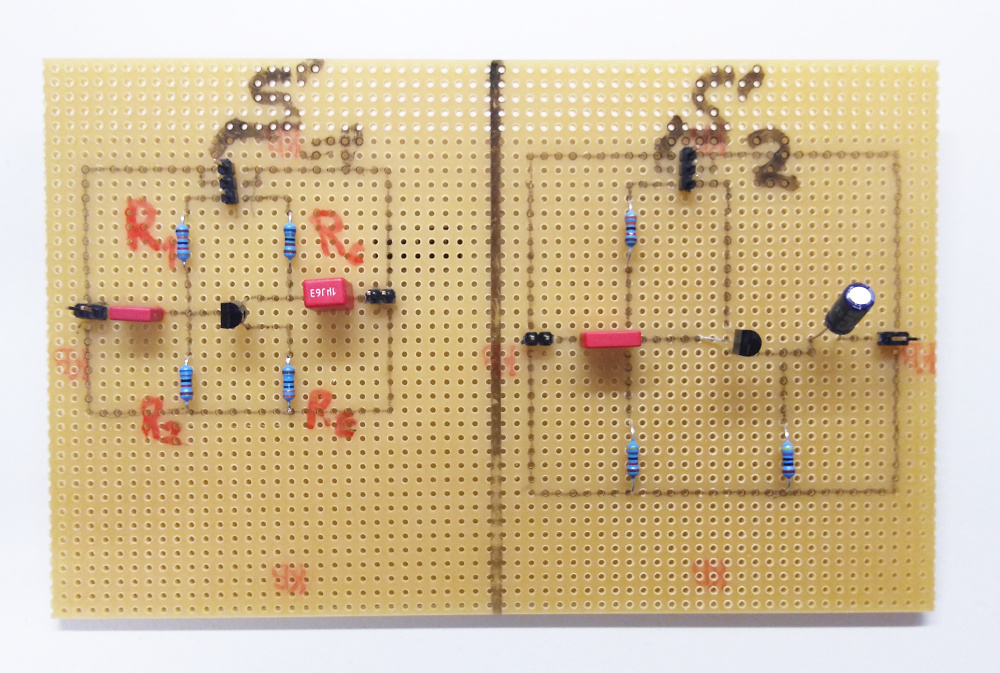
\includegraphics[]{jpg/FotoTransistorschaltungen}
        \end{adjustbox}
        \captionof{figure}{Foto unseres Aufbaus der Schaltung eines Transistors in Emitterschaltung mit Stromgegenkopplung (links) beziehungsweise in Kollektorschaltung (rechts)}
        \label{fig:FotoTransistorschaltungen}
    \end{center}
\endminipage
%
\subsubsection*{Inbetriebnahme und Messung der Kenngrößen}
%
Am Labornetzteil stellen wir eine Spannung von $\SI{15,0}{\volt}$ ein.
Die Skala hat eine Auflösung von $\SI{0,1}{\volt}$.
Es sind keine Schwankungen der eingestellten Spannung zu beobachten.
%
\par
%
Mit einem Multimeter messen wir mehrere verschiedene Spannungen.
Die Werte sind in Tabelle \ref{tab:MultimeterEmitterschaltung} eingetragen.
Als Messunsicherheit werden 5 Skalenteile gewählt.
Es sind keine Schwankungen der gemessenen Spannungen zu beobachten.
%
\par
%
\minipage{\linewidth}
    \begin{center}
        \captionsetup{type=table}
        \begin{adjustbox}{max width=\linewidth, keepaspectratio}
            \begin{tabular}{llllll}
            \toprule
            $U_{\text{CE}}$ [\SI{}{\volt}] & $U_{\text{BE}}$ [\SI{}{\volt}] & $U_{\text{C}}$ [\SI{}{\volt}] & $U_{R_1}$ [\SI{}{\volt}] & $U_{R_2}$ [\SI{}{\volt}] \\
            \midrule
            \SI{7,85 \pm 0,05}{}           & \SI{0,628 \pm 0,005}{}         & \SI{6,82 \pm 0,05}{}          & \SI{14,03 \pm 0,05}{}    & \SI{0,958 \pm 0,005}{}   \\
            \bottomrule
            \end{tabular}
        \end{adjustbox}
        \captionof{table}{Mit dem Multimeter gemessene Spannungen an der Schaltung des Transistors in Emitterschaltung}
        \label{tab:MultimeterEmitterschaltung}
    \end{center}
\endminipage
%
\subsubsection*{Verstärkung bei \SI{500}{\hertz}, Phasenunterschied und Untersuchung des Aussteuerbereichs}
%
Wir nehmen den Funktionsgenerator in Betrieb mit Frequenz $f = \SI{500}{\hertz}$ und Spitze-Spitze-Spannung von $V_{\text{PP}} = \SI{0,5}{\volt}$.
Am Oszilloskop wird Eingangs- und Ausgangssignal des Verstärkers angeschlossen.
Es ergibt sich eine Aufnahme wie in Abbildung \ref{fig:OsziEmitterschaltung} zu sehen.
%
\par
%
\minipage{\linewidth}
    \begin{center}
        \captionsetup{type=figure}
        \begin{adjustbox}{max width=\linewidth, keepaspectratio}
            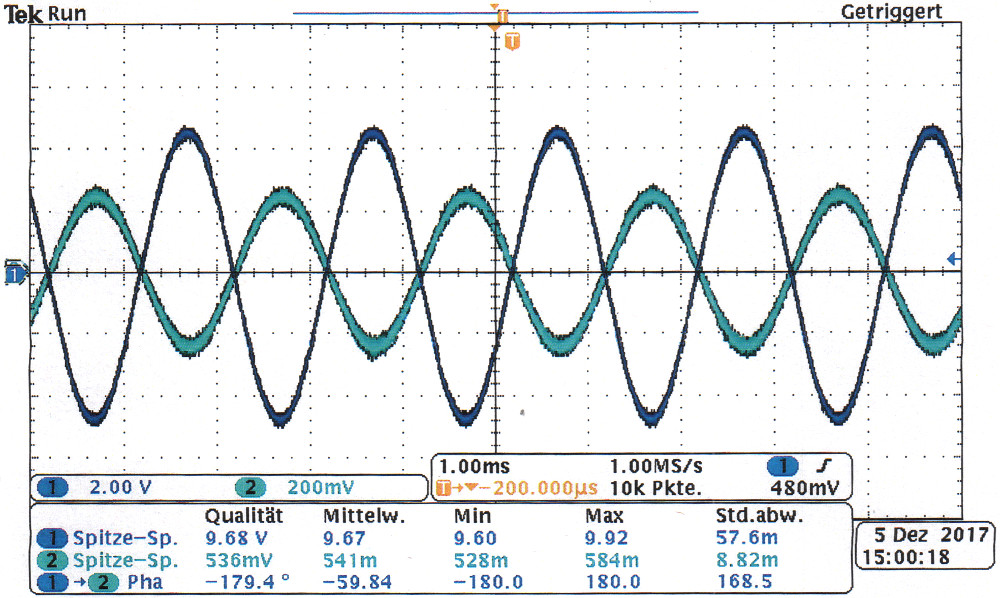
\includegraphics[width=120mm]{jpg/Emitterschaltung}
        \end{adjustbox}
        \captionof{figure}{Vergleich zwischen Eingangssignal (2) und Ausgangssignal (1) am Verstärker}
        \label{fig:OsziEmitterschaltung}
    \end{center}
\endminipage
%
\par
%
Mit der \enquote{Measure} Funktion des Oszilloskops werden die Spitze-Spitze-Spannungen der beiden Signale vermessen.
Die Messunsicherheiten werden aus den beobachteten Schwankungen geschätzt.
Die Ergebnisse sind in Tabelle \ref{tab:OsziEmitterschaltung} eingetragen.
%
\par
%
\minipage{\linewidth}
    \begin{center}
        \captionsetup{type=table}
        \begin{adjustbox}{max width=\linewidth, keepaspectratio}
            \begin{tabular}{ll}
            \toprule
            $U_{\text{SS}}$ des Eingangssignals & $U_{\text{SS}}$ des Ausgangssignals \\
            \midrule
            \SI{541 \pm 20}{\milli\volt}        & \SI{9,67 \pm 0,10}{\volt}           \\
            \bottomrule
            \end{tabular}
        \end{adjustbox}
        \captionof{table}{Mit dem Oszilloskop gemessene Spitze-Spitze-Spannungen}
        \label{tab:OsziEmitterschaltung}
    \end{center}
\endminipage
%
\par
%
Der Phasenunterschied zwischen den beiden Signalen kann ebenfalls mit dem Oszilloskop bestimmt werden.
Das Oszilloskop lässt dabei Werte von \SIrange{-180}{180}{\degree} zu.
Aufgrund von Schwankungen werden Werte von \SIrange{-178}{-180}{\degree} beziehungsweise von \SIrange{178}{180}{\degree} angezeigt.
Der in Abbildung \ref{fig:OsziEmitterschaltung} verzeichnete Mittelwert ist daher ohne Bedeutung und zu verwerfen.
%
\par
%
Bei einer qualitativen Untersuchung des Aussteuerbereichs lässt sich feststellen, dass ab $U_{\text{SS}} = \SI{0,85}{\volt}$ am Eingangssignal Verzerrungen im Ausgangssignal auftreten.
Es ergibt sich ein Plateau an den Extremstellen.
$U_{\text{SS}}$ des Ausgangssignals kann einen bestimmten Wert nicht überschreiten.
%
\subsubsection*{Messung des Frequenzgangs}
%
Für die Messung des Frequenzgangs notieren wir mehrere Werte für Frequenz $f$ sowie Spitze-Spitze-Spannungen $U_{\text{SS}}$ des Eingangssignals und des Ausgangssignals.
Die Ergebnisse sind in Tabelle \ref{tab:FrequenzgangEmitterschaltung} eingetragen.
In diesem Versuchsteil wurde $U_{\text{SS}}$ des Eingangssignals nur einmalig am Anfang notiert und hat sich im weiteren Verlauf nicht bedeutend geändert.
%
\par
%
\minipage{\linewidth}
    \begin{center}
        \captionsetup{type=table}
        \begin{adjustbox}{max width=\linewidth, keepaspectratio}
            \begin{tabular}{lll}
            \toprule
            Frequenz $f$ [\SI{}{\hertz}] & $U_{\text{SS}}$ des Eingangssignals [\SI{}{\volt}] & $U_{\text{SS}}$ des Ausgangssignals [\SI{}{\volt}] \\
            \midrule
            \SI{10}{}                    & \SI{0,541 \pm 0,02}{}                              & \SI{2,58 \pm 0,10}{}                               \\
            \SI{20}{}                    & $\sim$                                             & \SI{4,50 \pm 0,10}{}                               \\
            \SI{30}{}                    & $\sim$                                             & \SI{5,92 \pm 0,10}{}                               \\
            \SI{40}{}                    & $\sim$                                             & \SI{6,96 \pm 0,10}{}                               \\
            \SI{50}{}                    & $\sim$                                             & \SI{7,60 \pm 0,10}{}                               \\
            \SI{60}{}                    & $\sim$                                             & \SI{8,08 \pm 0,10}{}                               \\
            \SI{70}{}                    & $\sim$                                             & \SI{8,40 \pm 0,10}{}                               \\
            \SI{80}{}                    & $\sim$                                             & \SI{8,72 \pm 0,10}{}                               \\
            \SI{90}{}                    & $\sim$                                             & \SI{8,88 \pm 0,10}{}                               \\
            \SI{100}{}                   & $\sim$                                             & \SI{9,04 \pm 0,10}{}                               \\
            \SI{110}{}                   & $\sim$                                             & \SI{9,12 \pm 0,10}{}                               \\
            \SI{120}{}                   & $\sim$                                             & \SI{9,20 \pm 0,10}{}                               \\
            \SI{130}{}                   & $\sim$                                             & \SI{9,28 \pm 0,10}{}                               \\
            \SI{140}{}                   & $\sim$                                             & \SI{9,36 \pm 0,10}{}                               \\
            \SI{150}{}                   & $\sim$                                             & \SI{9,36 \pm 0,10}{}                               \\
            \SI{1000}{}                  & $\sim$                                             & \SI{9,68 \pm 0,10}{}                               \\
            \SI{2000}{}                  & $\sim$                                             & \SI{9,68 \pm 0,10}{}                               \\
            \SI{3000}{}                  & $\sim$                                             & \SI{9,68 \pm 0,10}{}                               \\
            \SI{10000}{}                 & $\sim$                                             & \SI{9,68 \pm 0,10}{}                               \\
            \SI{20000}{}                 & $\sim$                                             & \SI{9,68 \pm 0,10}{}                               \\
            \SI{30000}{}                 & $\sim$                                             & \SI{9,60 \pm 0,10}{}                               \\
            \SI{40000}{}                 & $\sim$                                             & \SI{9,60 \pm 0,10}{}                               \\
            \SI{50000}{}                 & $\sim$                                             & \SI{9,52 \pm 0,10}{}                               \\
            \SI{60000}{}                 & $\sim$                                             & \SI{9,36 \pm 0,10}{}                               \\
            \SI{70000}{}                 & $\sim$                                             & \SI{9,28 \pm 0,10}{}                               \\
            \SI{80000}{}                 & $\sim$                                             & \SI{9,12 \pm 0,10}{}                               \\
            \SI{90000}{}                 & $\sim$                                             & \SI{9,04 \pm 0,10}{}                               \\
            \SI{100000}{}                & $\sim$                                             & \SI{8,96 \pm 0,10}{}                               \\
            \bottomrule
            \end{tabular}
        \end{adjustbox}
        \captionof{table}{Mit dem Oszilloskop gemessene Werte für den Frequenzgang der Emitterschaltung}
        \label{tab:FrequenzgangEmitterschaltung}
    \end{center}
\endminipage
%
\subsubsection*{Temporäre Verbesserung der Schaltung durch Gleichstromgegenkopplung}
%
Parallel zum Widerstand $R_E$ wird ein Elektrolyt-Kondensator mit einer Kapazität von \SI{100}{\micro\farad} in die bestehende Schaltung eingebaut.
Am Funktionsgenerator wird eine Frequenz von etwa \SI{5}{\kilo\hertz} eingestellt.
Die Verstärkung von Ausgangs- zu Eingangsamplitude beträgt nun etwa \SI{100}{}.
Anschließend wird der Kondensator wieder entfernt.
%
\subsubsection*{Messung des Eingangs- und Ausgangswiderstands}
%
Am Funktionsgenerator ist Frequenz $f = \SI{1}{\kilo\hertz}$ und Spitze-Spitze-Spannung $V_{\text{PP}} = \SI{500}{\milli\volt}$ eingestellt.
Mit dem Oszilloskop messen wir eine Spitze-Spitze-Spannung von $U_{\text{SS}} = \SI{0,544 \pm 0,02}{\volt}$ für das Eingangssignal und $U_{\text{SS}} = \SI{9,68 \pm 0,10}{\volt}$ für das Ausgangssignal.
%
\par
%
Wir schalten zur Bestimmung von Eingangs- und Ausgangswiderstand ein Potentiometer hinzu wie in Abbildung \ref{fig:EinUndAusgangswiderstand} zu sehen.
Der Widerstand des Potentiometers wird variiert bis nur noch die halbe Spitze-Spitze-Spannung von $U_{\text{SS}} = \SI{4,80 \pm 0,10}{\volt}$ gemessen wird.
In der jeweiligen Konfiguration erhalten wir für den Eingangswiderstand $R_{\text{Ein}} = \SI{45,4 \pm 1,0}{\kilo\ohm}$ und für den Ausgangswiderstand $R_{\text{Aus}} = \SI{5,8 \pm 1,0}{\kilo\ohm}$.
Die Messunsicherheit wird dabei dadurch abgeschätzt, dass das Potentiometer mehrfach frisch eingestellt wird und entstehende Abweichungen betrachtet werden.
%
\par
%
\minipage{\linewidth}
    \begin{center}
        \captionsetup{type=figure}
        \begin{adjustbox}{max width=\linewidth, keepaspectratio}
            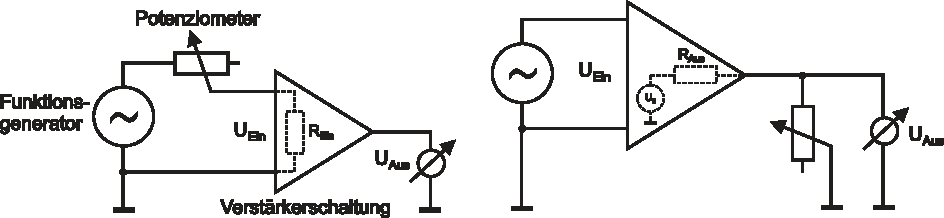
\includegraphics[]{pdf/EinUndAusgangswiderstand}
        \end{adjustbox}
        \captionof{figure}{Schaltung zur Bestimmung des Eingangswiderstands (links) beziehungsweise Ausgangswiderstands (rechts) (Quelle \cite{Anleitung})}
        \label{fig:EinUndAusgangswiderstand}
    \end{center}
\endminipage
%
\subsection{Verstärkerschaltung mit einem Transistor in Kollektorschaltung}
%
\subsubsection*{Dimensionierung}
%
Die berechnete Dimensionierung laut Tabelle \ref{tab:DimensionierungKollektorschaltung} wurden mit dem Versuchsbetreuer besprochen, abgeglichen und können verwendet werden.
%
\subsubsection*{Aufbau}
%
Wir bauen die Schaltung eines Transistors in Kollektorschaltung auf wie in Abbildung \ref{fig:Kollektorschaltung} zu sehen.
Die fertige Schaltung ist in Abbildung \ref{fig:FotoTransistorschaltungen} dargestellt.
%
\par
%
\minipage{\linewidth}
    \begin{center}
        \captionsetup{type=figure}
        \begin{adjustbox}{max width=\linewidth, keepaspectratio}
            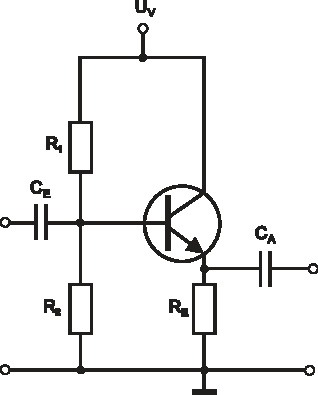
\includegraphics[]{pdf/Kollektorschaltung}
        \end{adjustbox}
        \captionof{figure}{Transistor in Kollektorschaltung (Quelle \cite{Anleitung})}
        \label{fig:Kollektorschaltung}
    \end{center}
\endminipage
%
\subsubsection*{Inbetriebnahme und Messung der Kenngrößen}
%
Analog des vorherigen Aufbaus werden verschiedene Spannungen notiert und in Tabelle \ref{tab:MultimeterKollektorschaltung} eingetragen.
%
\par
%
\minipage{\linewidth}
    \begin{center}
        \captionsetup{type=table}
        \begin{adjustbox}{max width=\linewidth, keepaspectratio}
            \begin{tabular}{llllll}
            \toprule
            $U_{\text{E}}$ [\SI{}{\volt}] & $U_{\text{BE}}$ [\SI{}{\volt}] & $U_{R_1}$ [\SI{}{\volt}] & $U_{R_2}$ [\SI{}{\volt}] \\
            \midrule
            \SI{7,56 \pm 0,05}{}          & \SI{0,660 \pm 0,005}{}         & \SI{6,70 \pm 0,05}{}     & \SI{8,25 \pm 0,05}{}     \\
            \bottomrule
            \end{tabular}
        \end{adjustbox}
        \captionof{table}{Mit dem Multimeter gemessene Spannungen an der Schaltung des Transistors in Kollektorschaltung}
        \label{tab:MultimeterKollektorschaltung}
    \end{center}
\endminipage
%
\subsubsection*{Verstärkung bei \SI{5}{\kilo\hertz} und Phasenunterschied}
%
Am Funktionsgenerator ist Frequenz $f = \SI{5}{\kilo\hertz}$ und Spitze-Spitze-Spannung $V_{\text{PP}} = \SI{1,0000}{\volt}$ eingestellt.
Die Aufnahmen mit dem Oszilloskop sind in Abbildung \ref{fig:Kollektorschaltung} beziehungsweise \ref{fig:Kollektorschaltung-absichtlich-verschoben} dargestellt.
Die Ergebnisse der Spannungsmessungen sind in Tabelle \ref{tab:OsziKollektorschaltung} eingetragen.
%
\par
%
\minipage{\linewidth}
    \begin{center}
        \captionsetup{type=figure}
        \begin{adjustbox}{max width=\linewidth, keepaspectratio}
            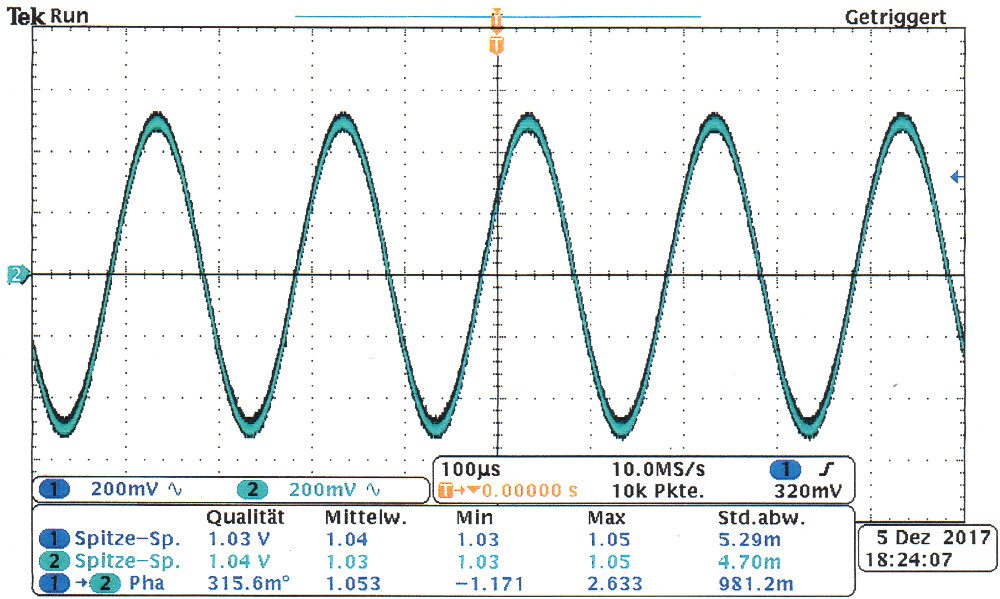
\includegraphics[width=120mm]{jpg/Kollektorschaltung}
        \end{adjustbox}
        \captionof{figure}{Vergleich zwischen Eingangssignal (2) und Ausgangssignal (1) am Verstärker}
        \label{fig:Kollektorschaltung}
    \end{center}
\endminipage
%
\par
%
\minipage{\linewidth}
    \begin{center}
        \captionsetup{type=figure}
        \begin{adjustbox}{max width=\linewidth, keepaspectratio}
            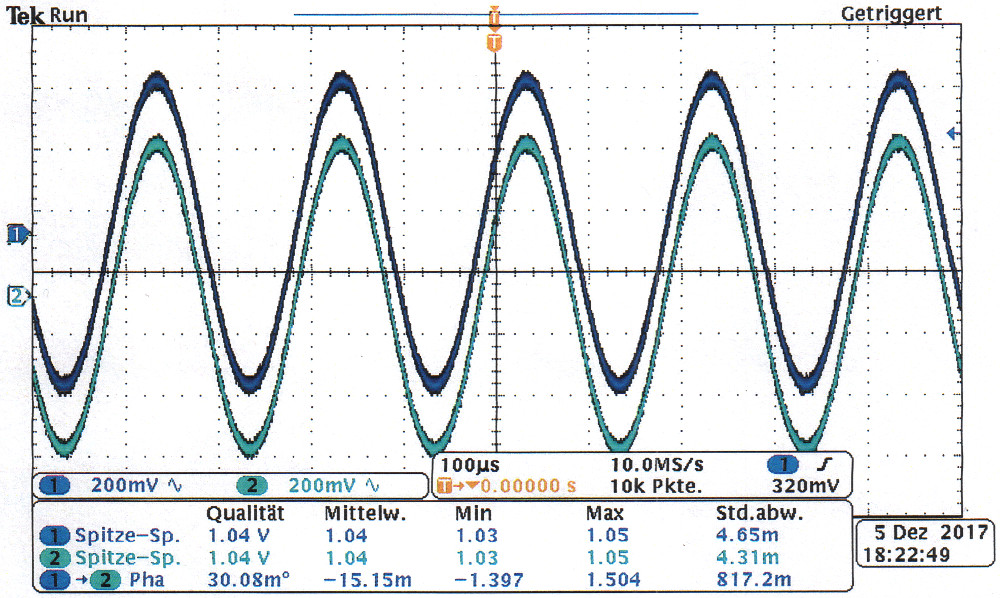
\includegraphics[width=120mm]{jpg/Kollektorschaltung-absichtlich-verschoben}
        \end{adjustbox}
        \captionof{figure}{Vergleich zwischen Eingangssignal (2) und Ausgangssignal (1) am Verstärker wobei im Vergleich zu Abbildung \ref{fig:Kollektorschaltung} absichtlich ein vertikales Offset eingestellt ist, da sonst beide Signale direkt übereinander liegen.}
        \label{fig:Kollektorschaltung-absichtlich-verschoben}
    \end{center}
\endminipage
%
\par
%
\minipage{\linewidth}
    \begin{center}
        \captionsetup{type=table}
        \begin{adjustbox}{max width=\linewidth, keepaspectratio}
            \begin{tabular}{ll}
            \toprule
            $U_{\text{SS}}$ des Eingangssignals & $U_{\text{SS}}$ des Ausgangssignals \\
            \midrule
            \SI{1,04 \pm 0,01}{\volt}           & \SI{1,03 \pm 0,01}{\volt}           \\
            \bottomrule
            \end{tabular}
        \end{adjustbox}
        \captionof{table}{Mit dem Oszilloskop gemessene Spitze-Spitze-Spannungen}
        \label{tab:OsziKollektorschaltung}
    \end{center}
\endminipage
%
\par
%
Der Phasenunterschied beträgt unter Berücksichtigung auftretender Schwankungen \SI{0 \pm 2}{\degree}.
%
\subsubsection*{Messung des Frequenzgangs}
%
Die Messung des Frequenzgangs verläuft analog zu der im vorhergehenden Versuchsteil.
Die Ergebnisse sind in Tabelle \ref{tab:FrequenzgangKollektorschaltung} eingetragen.
%
\par
%
\minipage{\linewidth}
    \begin{center}
        \captionsetup{type=table}
        \begin{adjustbox}{max width=\linewidth, keepaspectratio}
            \begin{tabular}{lll}
            \toprule
            Frequenz $f$ [\SI{}{\hertz}] & $U_{\text{SS}}$ des Eingangssignals [\SI{}{\milli\volt}] & $U_{\text{SS}}$ des Ausgangssignals [\SI{}{\milli\volt}] \\
            \midrule
            \SI{10}{}                    & \SI{848 \pm 10}{}                                        & \SI{240 \pm 10}{}                                        \\
            \SI{20}{}                    & \SI{984 \pm 10}{}                                        & \SI{464 \pm 10}{}                                        \\
            \SI{30}{}                    & \SI{1010 \pm 10}{}                                       & \SI{616 \pm 10}{}                                        \\
            \SI{40}{}                    & \SI{1020 \pm 10}{}                                       & \SI{728 \pm 10}{}                                        \\
            \SI{50}{}                    & \SI{1020 \pm 10}{}                                       & \SI{808 \pm 10}{}                                        \\
            \SI{60}{}                    & \SI{1030 \pm 10}{}                                       & \SI{864 \pm 10}{}                                        \\
            \SI{70}{}                    & \SI{1030 \pm 10}{}                                       & \SI{896 \pm 10}{}                                        \\
            \SI{80}{}                    & \SI{1030 \pm 10}{}                                       & \SI{920 \pm 10}{}                                        \\
            \SI{90}{}                    & \SI{1040 \pm 10}{}                                       & \SI{952 \pm 10}{}                                        \\
            \SI{100}{}                   & \SI{1040 \pm 10}{}                                       & \SI{968 \pm 10}{}                                        \\
            \SI{110}{}                   & \SI{1040 \pm 10}{}                                       & \SI{976 \pm 10}{}                                        \\
            \SI{120}{}                   & \SI{1030 \pm 10}{}                                       & \SI{992 \pm 10}{}                                        \\
            \SI{130}{}                   & \SI{1030 \pm 10}{}                                       & \SI{1000 \pm 10}{}                                       \\
            \SI{140}{}                   & \SI{1040 \pm 10}{}                                       & \SI{1010 \pm 10}{}                                       \\
            \SI{150}{}                   & \SI{1030 \pm 10}{}                                       & \SI{1000 \pm 10}{}                                       \\
            \SI{1000}{}                  & \SI{1040 \pm 10}{}                                       & \SI{1030 \pm 10}{}                                       \\
            \SI{2000}{}                  & \SI{1030 \pm 10}{}                                       & \SI{1030 \pm 10}{}                                       \\
            \SI{3000}{}                  & \SI{1030 \pm 10}{}                                       & \SI{1030 \pm 10}{}                                       \\
            \SI{10000}{}                 & \SI{1010 \pm 10}{}                                       & \SI{1000 \pm 10}{}                                       \\
            \SI{20000}{}                 & \SI{1000 \pm 10}{}                                       & \SI{1000 \pm 10}{}                                       \\
            \SI{30000}{}                 & \SI{1010 \pm 10}{}                                       & \SI{1000 \pm 10}{}                                       \\
            \SI{40000}{}                 & \SI{1020 \pm 10}{}                                       & \SI{1010 \pm 10}{}                                       \\
            \SI{140000}{}                & \SI{992 \pm 10}{}                                        & \SI{984 \pm 10}{}                                        \\
            \SI{240000}{}                & \SI{1000 \pm 10}{}                                       & \SI{1000 \pm 10}{}                                       \\
            \SI{340000}{}                & \SI{1020 \pm 10}{}                                       & \SI{1010 \pm 10}{}                                       \\
            \SI{440000}{}                & \SI{1010 \pm 10}{}                                       & \SI{1000 \pm 10}{}                                       \\
            \SI{540000}{}                & \SI{1010 \pm 10}{}                                       & \SI{1010 \pm 10}{}                                       \\
            \SI{640000}{}                & \SI{1020 \pm 10}{}                                       & \SI{1010 \pm 10}{}                                       \\
            \SI{740000}{}                & \SI{1010 \pm 10}{}                                       & \SI{1000 \pm 10}{}                                       \\
            \SI{840000}{}                & \SI{1010 \pm 10}{}                                       & \SI{1000 \pm 10}{}                                       \\
            \SI{940000}{}                & \SI{1010 \pm 10}{}                                       & \SI{1010 \pm 10}{}                                       \\
            \SI{1040000}{}               & \SI{1010 \pm 10}{}                                       & \SI{1000 \pm 10}{}                                       \\
            \bottomrule
            \end{tabular}
        \end{adjustbox}
        \captionof{table}{Mit dem Oszilloskop gemessene Werte für den Frequenzgang der Kollektorschaltung}
        \label{tab:FrequenzgangKollektorschaltung}
    \end{center}
\endminipage
%
\subsubsection*{Messung der Länge eines Koaxialkabels}
%
Der Funktionsgenerator liefert ein Rechtecksignal mit Frequenz $f = \SI{1}{\kilo\hertz}$.
Der Ausgang des Kollektorverstärkers wird an ein Koaxialkabel der Länge $L = \SI{20}{\meter}$ angeschlossen.
Am Oszilloskop wird sowohl das Signal vom Anfang als auch vom Ende des Kabels dargestellt.
Die Aufnahme ist in Abbildung \ref{fig:LaengenmessungKabelradar} zu sehen.
%
\par
%
\minipage{\linewidth}
    \begin{center}
        \captionsetup{type=figure}
        \begin{adjustbox}{max width=\linewidth, keepaspectratio}
            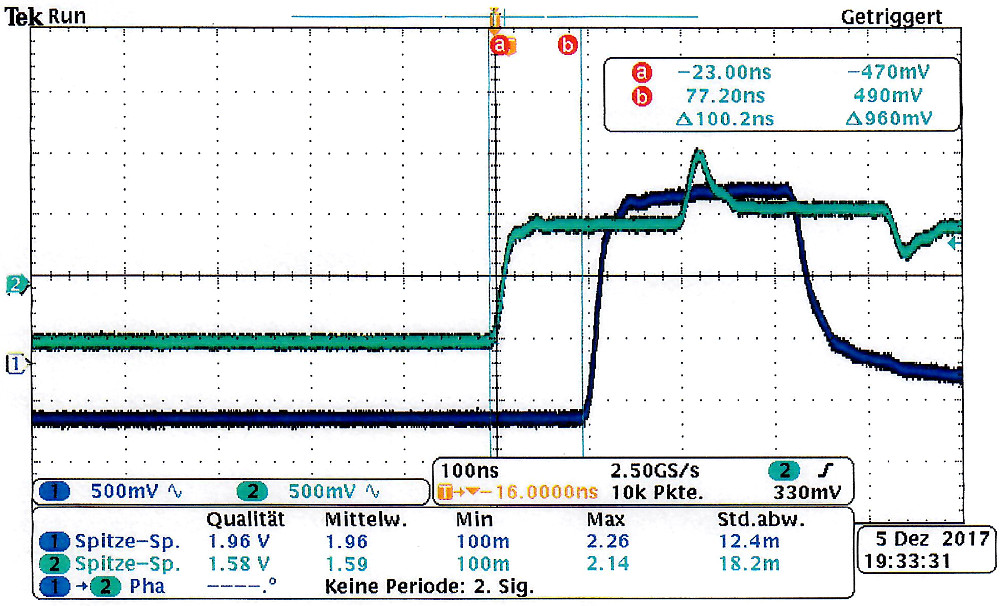
\includegraphics[width=120mm]{jpg/LaengenmessungKabelradar}
        \end{adjustbox}
        \captionof{figure}{Signal vom Anfang (2) und Ende (1) des Kabels}
        \label{fig:LaengenmessungKabelradar}
    \end{center}
\endminipage
%
\par
%
Der Ausgabe entnehmen wir einen Laufzeitunterschied von $t = \SI{100,2 \pm 2,0}{\nano\second}$.
%
\subsubsection*{Bestimmung der Wellenimpedanz eines Kabels}
%
Um die Impedanz eines Kabels zu bestimmen schalten wir parallel zum Oszilloskop über das Kabel ein Potentiometer.
Der Eingangswiderstand des Oszilloskops ist mit \SI{1}{\mega\ohm} angegeben.
Das verwendete Kabel hat eine Länge von \SI{13,5}{\meter} und eine theoretische Impedanz von \SI{50}{\ohm}.
%
\par
%
Zunächst erscheint das Signal wie in Abbildung \ref{fig:Impedanzmessung-ohne-Poti} dargestellt.
Der Widerstand des Potentiometers wird nun so lange variiert, bis die Schwingungen weitestgehend verschwinden.
Wir erhalten die Aufnahme wie in Abbildung \ref{fig:Impedanzmessung-mit-Poti} zu sehen.
Aufgrund großer Schwankungen beim Einstellen des Signals notieren wir den Widerstand des Potentiometers mit \SI{70 \pm 20}{\ohm}.
%
\par
%
\minipage{\linewidth}
    \begin{center}
        \captionsetup{type=figure}
        \begin{adjustbox}{max width=\linewidth, keepaspectratio}
            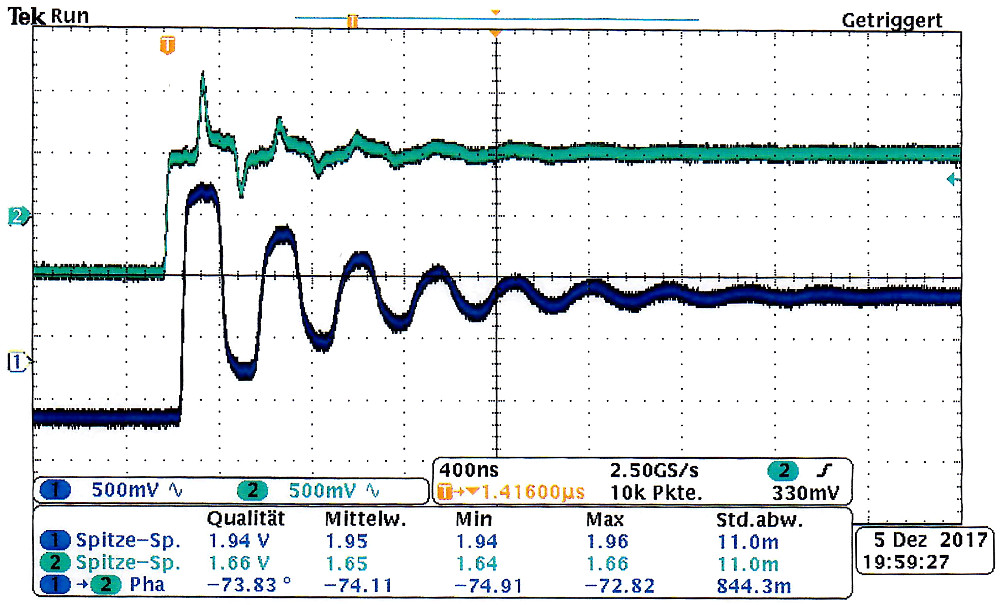
\includegraphics[width=120mm]{jpg/Impedanzmessung-ohne-Poti}
        \end{adjustbox}
        \captionof{figure}{Messung der Impedanz ohne passenden Widerstand durch das Potentiometer}
        \label{fig:Impedanzmessung-ohne-Poti}
    \end{center}
\endminipage
%
\par
%
\minipage{\linewidth}
    \begin{center}
        \captionsetup{type=figure}
        \begin{adjustbox}{max width=\linewidth, keepaspectratio}
            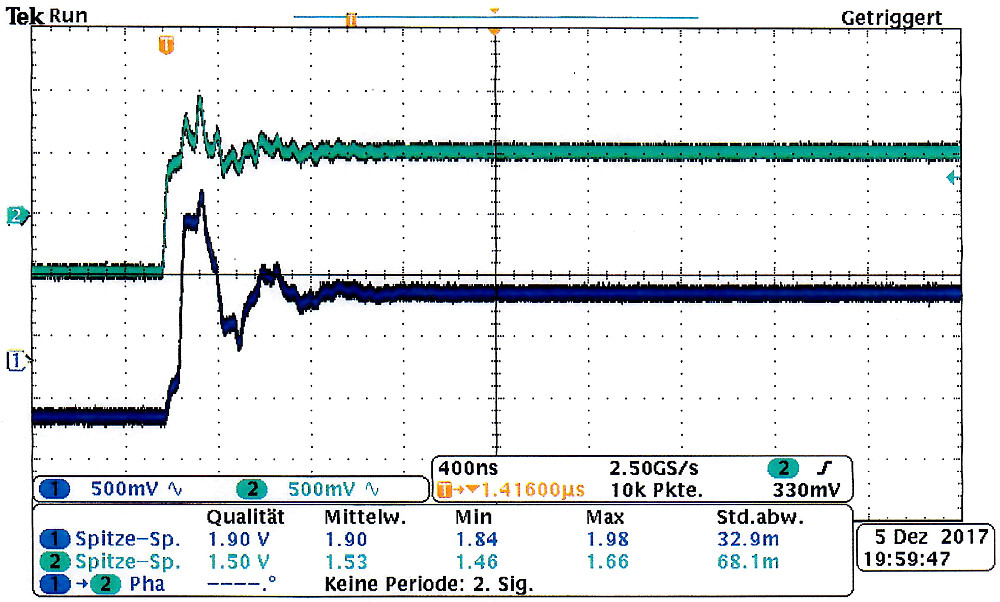
\includegraphics[width=120mm]{jpg/Impedanzmessung-mit-Poti}
        \end{adjustbox}
        \captionof{figure}{Messung der Impedanz mit passend eingestelltem Potentiometer}
        \label{fig:Impedanzmessung-mit-Poti}
    \end{center}
\endminipage
%
\subsection{Aufbau eines PID-Reglers zur Drehzahlregelung eines Motors}
%
\subsubsection*{Dimensionierung}
%
Die berechnete Dimensionierung laut Tabelle \ref{tab:DimensionierungPIDRegler} wurden mit dem Versuchsbetreuer besprochen, abgeglichen und können verwendet werden.
%
\subsubsection*{Aufbau}
%
Wir bauen die Schaltung eines PID-Reglers mithilfe der zur Verfügung gestellten Platine auf wie in der Versuchsanleitung \cite{Anleitung} beschrieben.
Die fertige Schaltung ist in Abbildung \ref{fig:FotoMotorregler} dargestellt.
%
\minipage{\linewidth}
    \begin{center}
        \captionsetup{type=figure}
        \begin{adjustbox}{max width=\linewidth, keepaspectratio}
            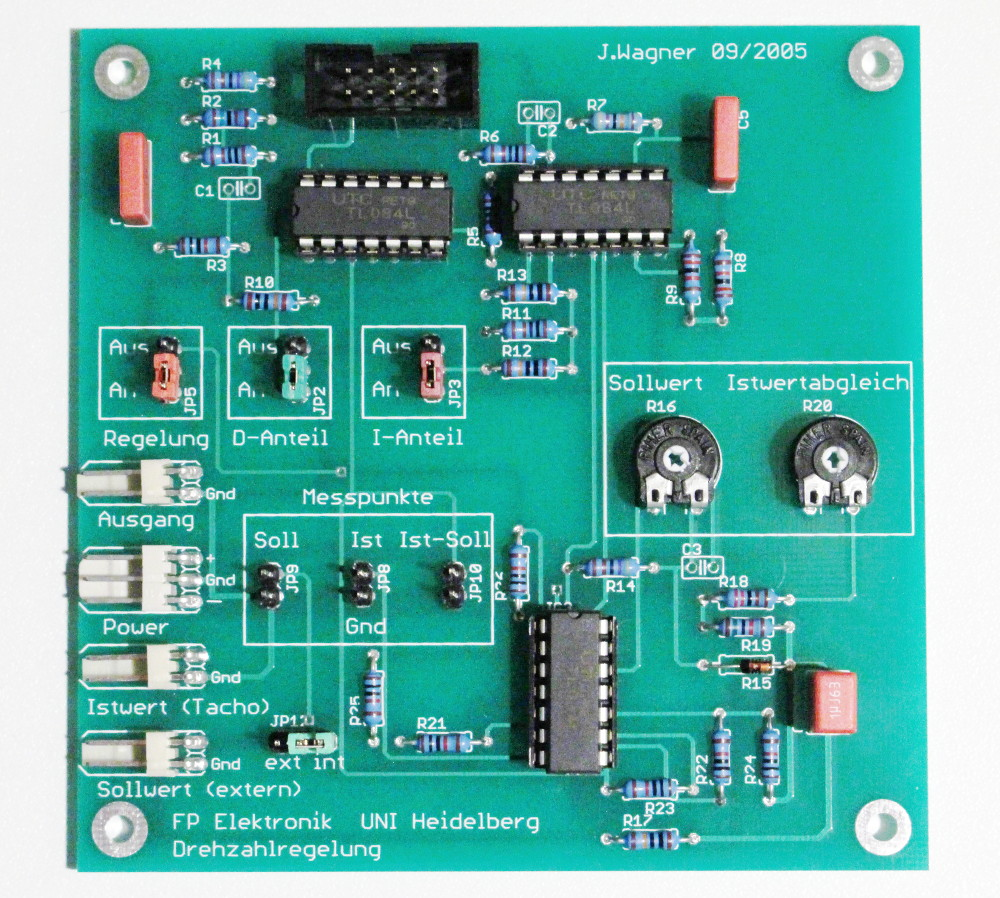
\includegraphics[width=120mm]{jpg/FotoMotorregler}
        \end{adjustbox}
        \captionof{figure}{Foto unseres Aufbaus der Schaltung eines PID-Reglers zur Drehzahlregelung eines Motors}
        \label{fig:FotoMotorregler}
    \end{center}
\endminipage
%
\subsubsection*{Inbetriebnahme mit interner Sollwert-Regelung}
%
Über die interne Sollwert-Regelung können wir durch Variieren des passenden Potentiometers korrespondierende Spannungen von \SI{240}{\milli\volt} bis \SI{7,12}{\volt} am Sollwert-Messpunkt einstellen.
Es sind keine Schwankungen der Werte zu beobachten.
%
\par
%
Mit angeschlossenem Tacho und eingeschaltetem Proportional-Regler erhalten wir einen Istwert ungleich Null.
Am Sollwert-Messpunkt können Spannungen von \SI{600}{\milli\volt} bis \SI{7,60}{\volt} verzeichnet werden - am Istwert-Messpunkt von \SI{160}{\milli\volt} bis \SI{5,76}{\volt}.
Wird der $K_{\text{P}}$-Wert erhöht, reagiert der Motor auch bei kleinen Sollwerten viel schneller.
Wir können den Motor insgesamt langsamer laufen lassen.
%
\subsubsection*{Externe Sollwert-Regelung und Einstellungen am Funktionsgenerator}
%
Für die weiteren Messungen verwenden wir aus Gründen der Reproduzierbarkeit nicht die interne Sollwert-Regelung sondern schließen stattdessen den Funktionsgenerator an die externe Sollwert-Regelung an.
Um ein Signal wie in Abbildung \ref{fig:Rechtecksignal} dargestellt zu erhalten, stellen wir am Funktionsgenerator eine Rechteckspannung mit Frequenz $\SI{200}{\milli\hertz}$, Amplitude $\SI{4,000}{\volt}$ und Offset $\SI{3,000}{\volt}$ ein.
%
\par
%
\minipage{\linewidth}
    \begin{center}
        \captionsetup{type=figure}
        \begin{adjustbox}{max width=\linewidth, keepaspectratio}
            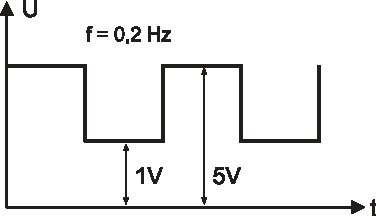
\includegraphics[]{pdf/Rechtecksignal}
        \end{adjustbox}
        \captionof{figure}{Rechtecksignal des Funktionsgenerators}
        \label{fig:Rechtecksignal}
    \end{center}
\endminipage
%
\par
%
Ohne Regelung erhalten wir die Aufnahme wie in Abbildung \ref{fig:Sinus-Regler-aus} dargestellt.
Für verschiedene Einstellungen der Regelparameter beobachten wir unterschiedliche Reaktionen auf die Sollwert-Änderungen.
Für eine weitere Untersuchung betrachten wir im Folgenden P-Regelung, PI-Regelung, PD-Regelung und PID-Regelung genauer.
%
\par
%
\minipage{\linewidth}
    \begin{center}
        \captionsetup{type=figure}
        \begin{adjustbox}{max width=\linewidth, keepaspectratio}
            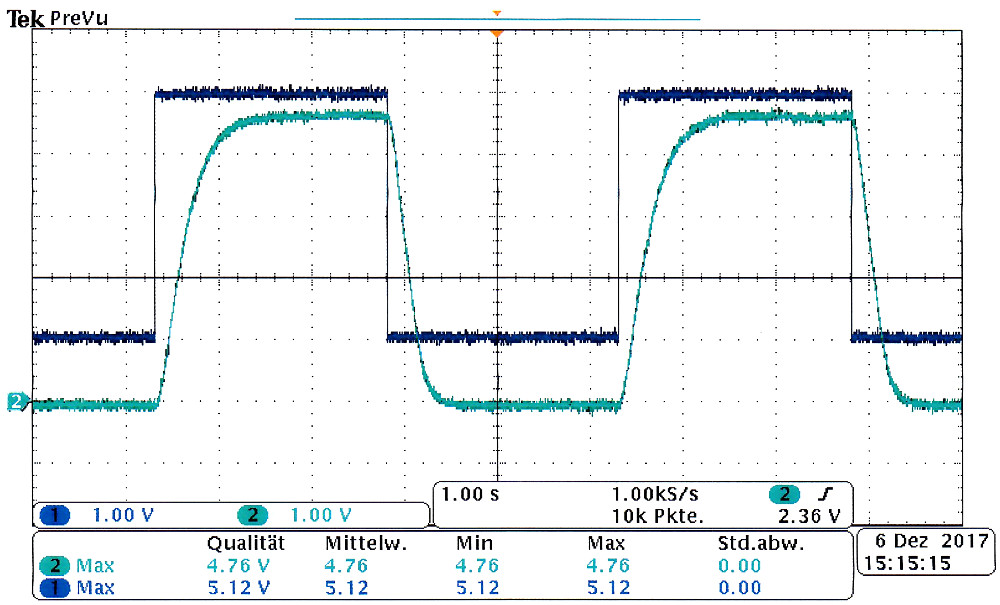
\includegraphics[width=120mm]{jpg/Sinus-Regler-aus}
        \end{adjustbox}
        \captionof{figure}{Sollwert (1) und Istwert (2) der Motorsteuerung ohne eingeschaltete P-, I- oder D-Regelung}
        \label{fig:Sinus-Regler-aus}
    \end{center}
\endminipage
%
\subsubsection*{Untersuchung P-Regelung}
%
Wir untersuchen $K_{\text{P}}$ mit verschiedenen Einstellungen des Potentiometers wie in Abbildungen \ref{fig:Sinus-KP-0-Skt}, \ref{fig:Sinus-KP-5-Skt}, \ref{fig:Sinus-KP-10-Skt} und \ref{fig:Sinus-KP-50-Skt} zu sehen.
Für kleines $K_{\text{P}}$ erkennen wir eine große stationäre Regelabweichung sowie geringe Stabilität des Istwerts durch andauernde Schwingungen.
Diese Schwingungen, sowie die stationäre Regelabweichung nehmen mit zunehmenden $K_{\text{P}}$ ab.
Es treten dann allerdings zunehmend Überschwingungen bei jeder Sollwertänderung auf, die den Istwert zunächst um den Sollwert oszillieren lassen bevor er sich annähert.
Die Flanke steigt/fällt für große $K_{\text{P}}$ etwas steiler als für niedrige Werte.
%
\par
%
\minipage{\linewidth}
    \begin{center}
        \captionsetup{type=figure}
        \begin{adjustbox}{max width=\linewidth, keepaspectratio}
            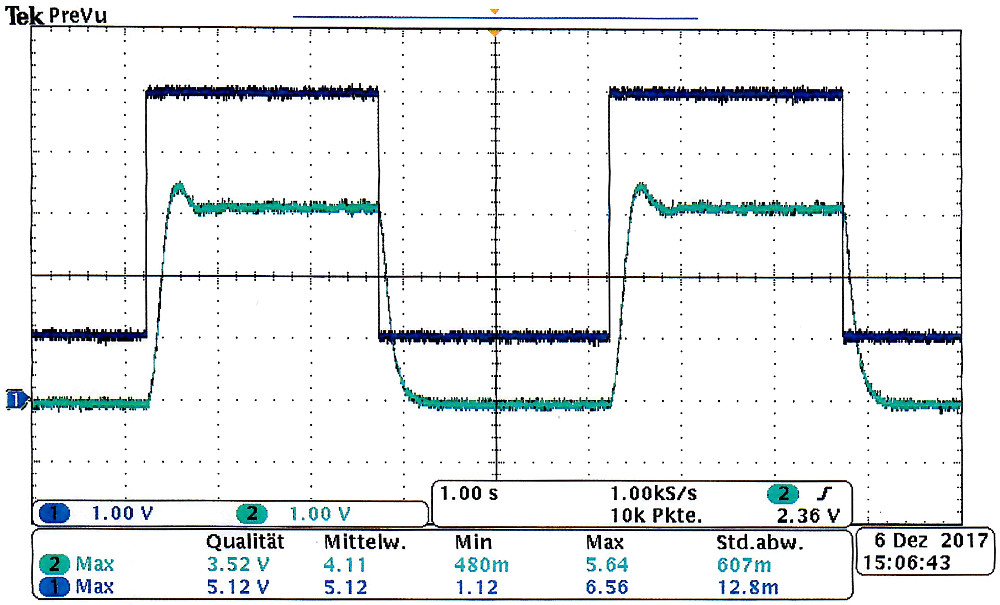
\includegraphics[width=120mm]{jpg/Sinus-KP-0-Skt}
        \end{adjustbox}
        \captionof{figure}{Sollwert (1) und Istwert (2) einer P-Regelung mit $K_{\text{P}} = \SI{0}{Skt}$}
        \label{fig:Sinus-KP-0-Skt}
    \end{center}
\endminipage
%
\par
%
\minipage{\linewidth}
    \begin{center}
        \captionsetup{type=figure}
        \begin{adjustbox}{max width=\linewidth, keepaspectratio}
            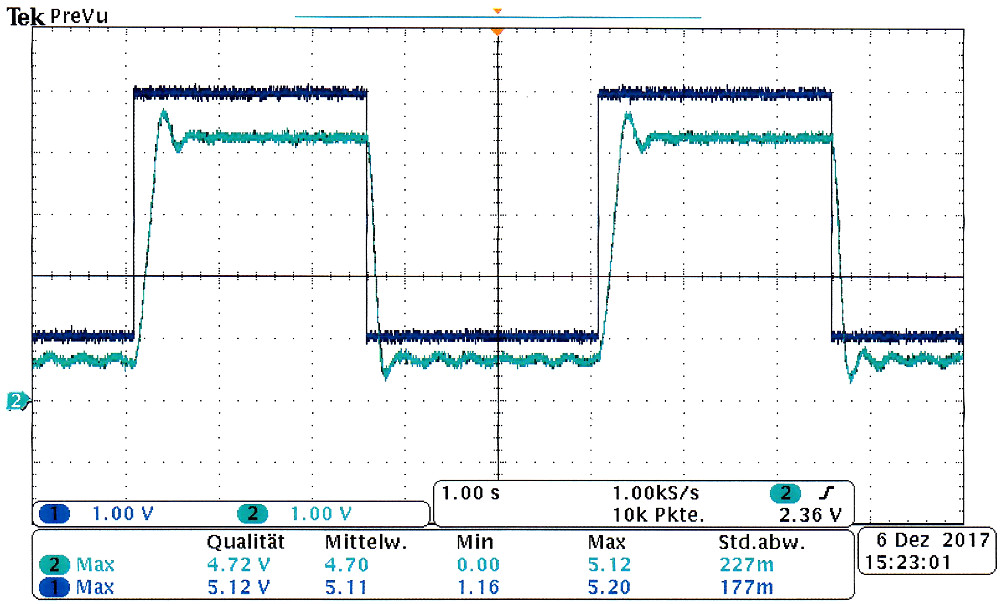
\includegraphics[width=120mm]{jpg/Sinus-KP-5-Skt}
        \end{adjustbox}
        \captionof{figure}{Sollwert (1) und Istwert (2) einer P-Regelung mit $K_{\text{P}} = \SI{5}{Skt}$}
        \label{fig:Sinus-KP-5-Skt}
    \end{center}
\endminipage
%
\par
%
\minipage{\linewidth}
    \begin{center}
        \captionsetup{type=figure}
        \begin{adjustbox}{max width=\linewidth, keepaspectratio}
            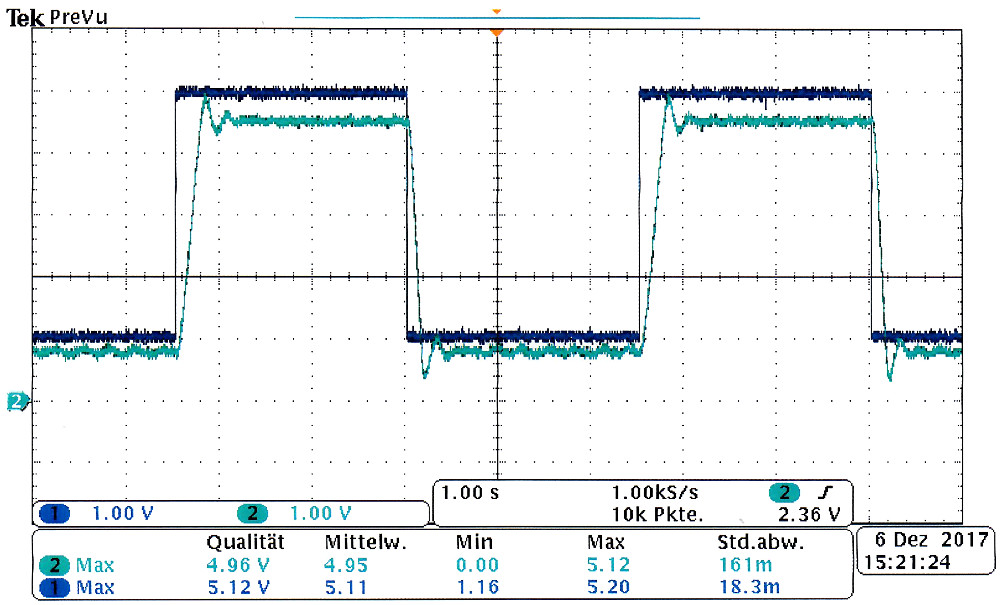
\includegraphics[width=120mm]{jpg/Sinus-KP-10-Skt}
        \end{adjustbox}
        \captionof{figure}{Sollwert (1) und Istwert (2) einer P-Regelung mit $K_{\text{P}} = \SI{10}{Skt}$}
        \label{fig:Sinus-KP-10-Skt}
    \end{center}
\endminipage
%
\par
%
\minipage{\linewidth}
    \begin{center}
        \captionsetup{type=figure}
        \begin{adjustbox}{max width=\linewidth, keepaspectratio}
            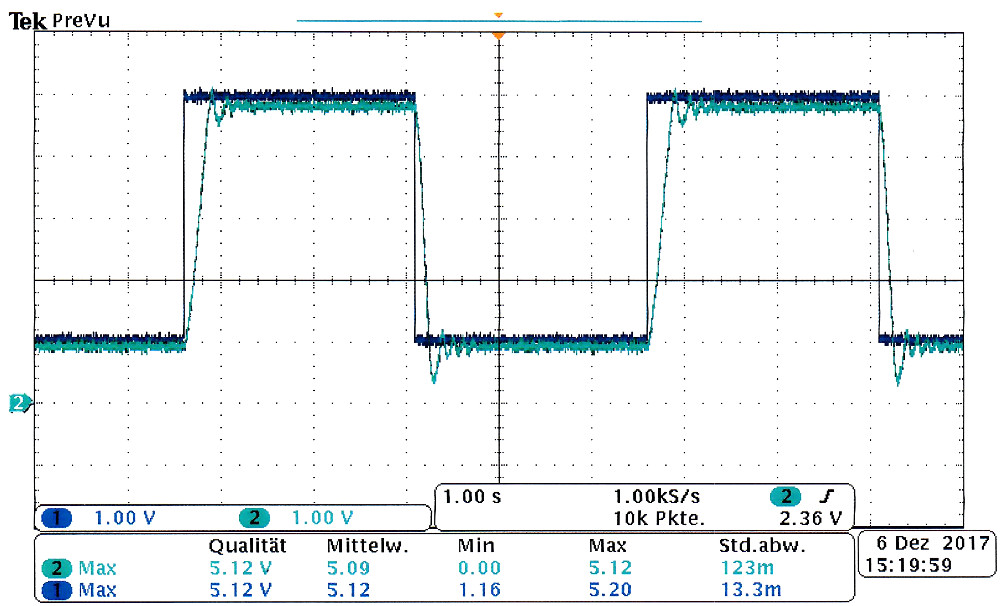
\includegraphics[width=120mm]{jpg/Sinus-KP-50-Skt}
        \end{adjustbox}
        \captionof{figure}{Sollwert (1) und Istwert (2) einer P-Regelung mit $K_{\text{P}} = \SI{50}{Skt}$}
        \label{fig:Sinus-KP-50-Skt}
    \end{center}
\endminipage
%
\par
%
Zusätzlich nehmen wir für einen kleinen sowie für einen großen Wert von $K_{\text{P}}$ den Messpunkt Ist-Soll auf und erhalten Abbildungen \ref{fig:Sinus-KP-0-Skt-Ist-Soll-Differenz} und \ref{fig:Sinus-KP-50-Skt-Ist-Soll-Differenz}.
%
\par
%
\minipage{\linewidth}
    \begin{center}
        \captionsetup{type=figure}
        \begin{adjustbox}{max width=\linewidth, keepaspectratio}
            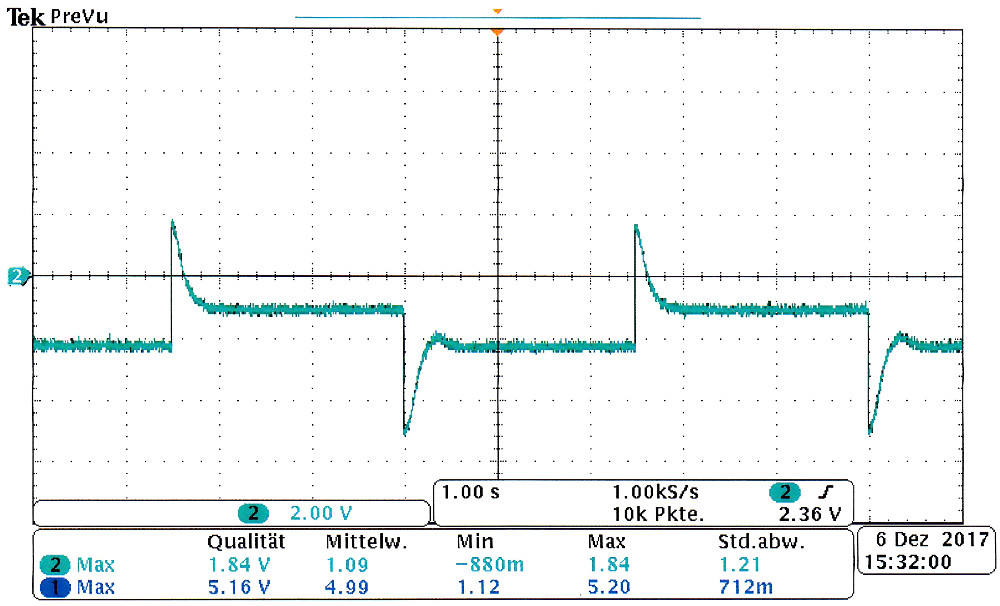
\includegraphics[width=120mm]{jpg/Sinus-KP-0-Skt-Ist-Soll-Differenz}
        \end{adjustbox}
        \captionof{figure}{Messpunkt Ist-Soll einer P-Regelung mit $K_{\text{P}} = \SI{0}{Skt}$}
        \label{fig:Sinus-KP-0-Skt-Ist-Soll-Differenz}
    \end{center}
\endminipage
%
\par
%
\minipage{\linewidth}
    \begin{center}
        \captionsetup{type=figure}
        \begin{adjustbox}{max width=\linewidth, keepaspectratio}
            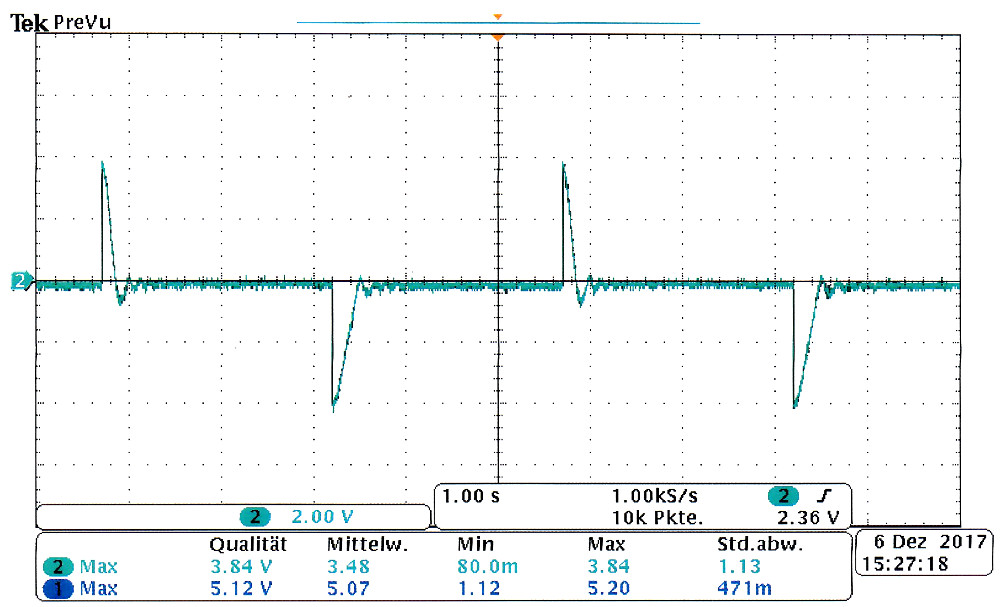
\includegraphics[width=120mm]{jpg/Sinus-KP-50-Skt-Ist-Soll-Differenz}
        \end{adjustbox}
        \captionof{figure}{Messpunkt Ist-Soll einer P-Regelung mit $K_{\text{P}} = \SI{50}{Skt}$}
        \label{fig:Sinus-KP-50-Skt-Ist-Soll-Differenz}
    \end{center}
\endminipage
%
\subsubsection*{Untersuchung PI-Regelung}
%
Wir schalten den I-Regler ein, sodass nun P- und I-Regler aktiv sind.
Beide Regelparameter werden zunächst auf \SI{0}{Skt} eingestellt.
Die Regelgeschwindigkeit nimmt im Vergleich zur P-Regelung ab, wir erkennen deutlich größere Überschwingungen.
Dies verstärkt sich mit zunehmendem $K_{\text{I}}$, wie in Abbildungen \ref{fig:Sinus-KP-klein-KI-klein}, \ref{fig:Sinus-KP-klein-KI-gross}, \ref{fig:Sinus-KP-gross-KI-gross} und \ref{fig:Sinus-KP-gross-KI-klein} zu sehen.
%
\par
%
\minipage{\linewidth}
    \begin{center}
        \captionsetup{type=figure}
        \begin{adjustbox}{max width=\linewidth, keepaspectratio}
            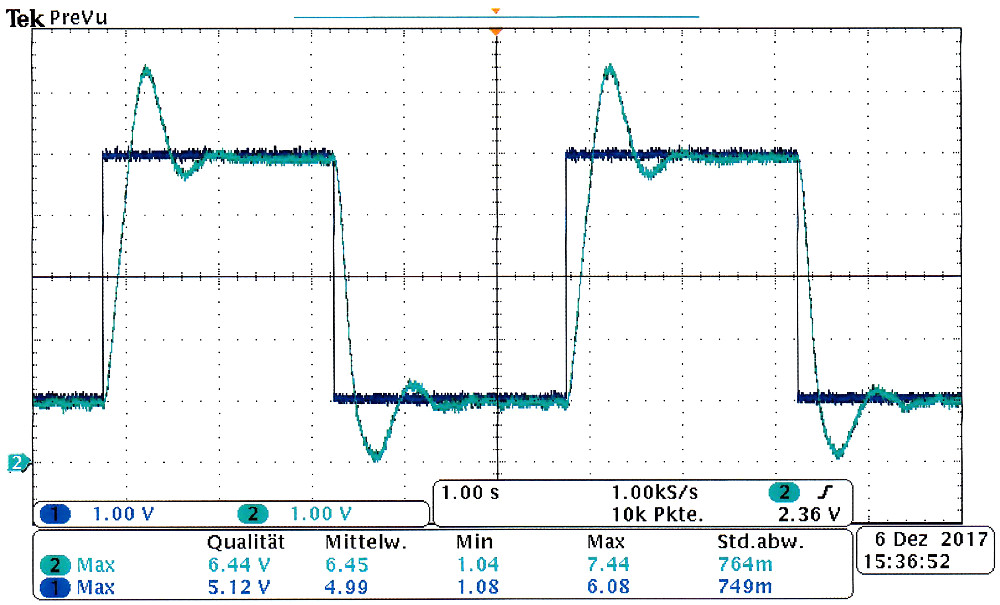
\includegraphics[width=120mm]{jpg/Sinus-KP-klein-KI-klein}
        \end{adjustbox}
        \captionof{figure}{PI-Regelung mit kleinem $K_{\text{P}}$ und kleinem $K_{\text{I}}$}
        \label{fig:Sinus-KP-klein-KI-klein}
    \end{center}
\endminipage
%
\par
%
\minipage{\linewidth}
    \begin{center}
        \captionsetup{type=figure}
        \begin{adjustbox}{max width=\linewidth, keepaspectratio}
            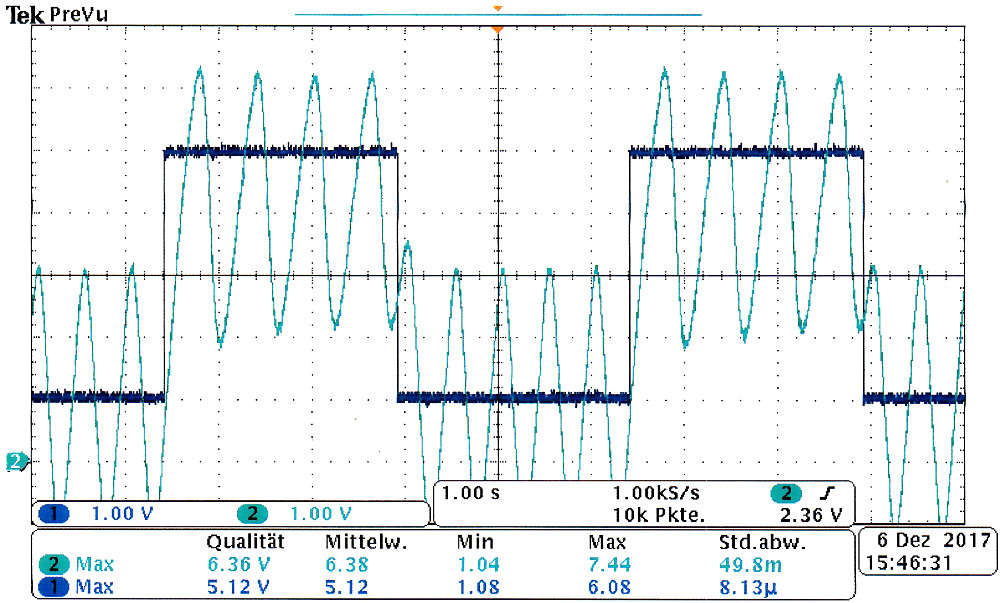
\includegraphics[width=120mm]{jpg/Sinus-KP-klein-KI-gross}
        \end{adjustbox}
        \captionof{figure}{PI-Regelung mit kleinem $K_{\text{P}}$ und großem $K_{\text{I}}$}
        \label{fig:Sinus-KP-klein-KI-gross}
    \end{center}
\endminipage
%
\par
%
\minipage{\linewidth}
    \begin{center}
        \captionsetup{type=figure}
        \begin{adjustbox}{max width=\linewidth, keepaspectratio}
            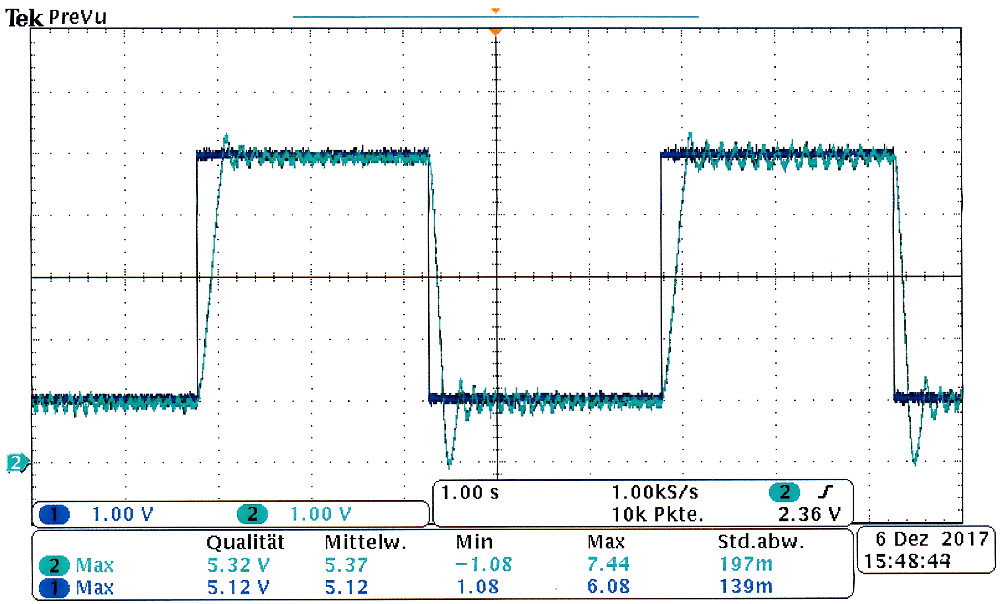
\includegraphics[width=120mm]{jpg/Sinus-KP-gross-KI-gross}
        \end{adjustbox}
        \captionof{figure}{PI-Regelung mit großem $K_{\text{P}}$ und großem $K_{\text{I}}$}
        \label{fig:Sinus-KP-gross-KI-gross}
    \end{center}
\endminipage
%
\par
%
\minipage{\linewidth}
    \begin{center}
        \captionsetup{type=figure}
        \begin{adjustbox}{max width=\linewidth, keepaspectratio}
            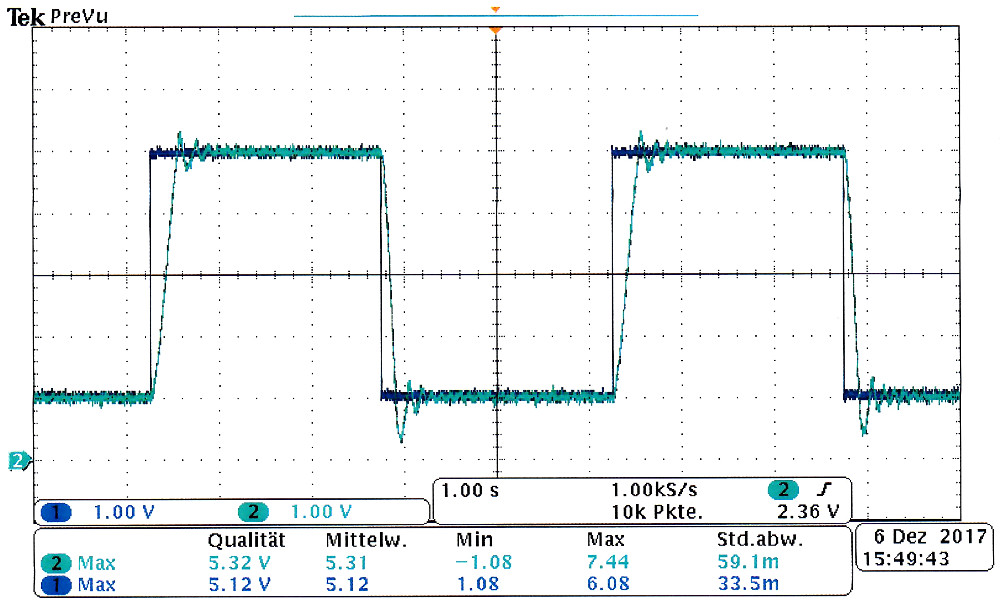
\includegraphics[width=120mm]{jpg/Sinus-KP-gross-KI-klein}
        \end{adjustbox}
        \captionof{figure}{PI-Regelung mit großem $K_{\text{P}}$ und kleinem $K_{\text{I}}$}
        \label{fig:Sinus-KP-gross-KI-klein}
    \end{center}
\endminipage
%
\subsubsection*{Untersuchung PD-Regelung}
%
Die I-Regelung wird entfernt und stattdessen die D-Regelung hinzugefügt.
Es sind nun P- und D-Regler aktiv.
Wir untersuchen qualitativ die Fälle für $K_{\text{P}}$ groß und klein in Kombination mit $K_{\text{D}}$ groß und klein, wie in Abbildungen \ref{fig:Sinus-KP-klein-KD-klein}, \ref{fig:Sinus-KP-klein-KD-gross}, \ref{fig:Sinus-KP-gross-KD-gross} und \ref{fig:Sinus-KP-gross-KD-klein} dargestellt.
Der $K_{\text{D}}$ Parameter sorgt dafür, dass Schwingungen zu Beginn der Istwertanpassung ausbleiben.
Wird diese Funktion allerdings übermäßig genutzt, also $K_{\text{D}}$ zu groß gewählt, können wir eine zu flach verlaufende Flanke bei der Anpassung beobachten.
%
\par
%
\minipage{\linewidth}
    \begin{center}
        \captionsetup{type=figure}
        \begin{adjustbox}{max width=\linewidth, keepaspectratio}
            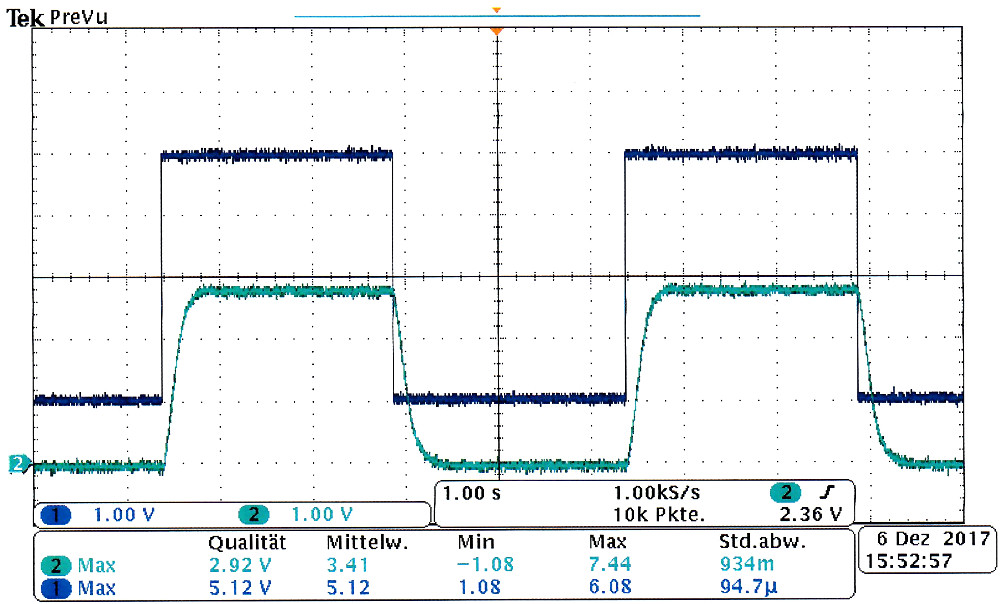
\includegraphics[width=120mm]{jpg/Sinus-KP-klein-KD-klein}
        \end{adjustbox}
        \captionof{figure}{PD-Regelung mit kleinem $K_{\text{P}}$ und kleinem $K_{\text{D}}$}
        \label{fig:Sinus-KP-klein-KD-klein}
    \end{center}
\endminipage
%
\par
%
\minipage{\linewidth}
    \begin{center}
        \captionsetup{type=figure}
        \begin{adjustbox}{max width=\linewidth, keepaspectratio}
            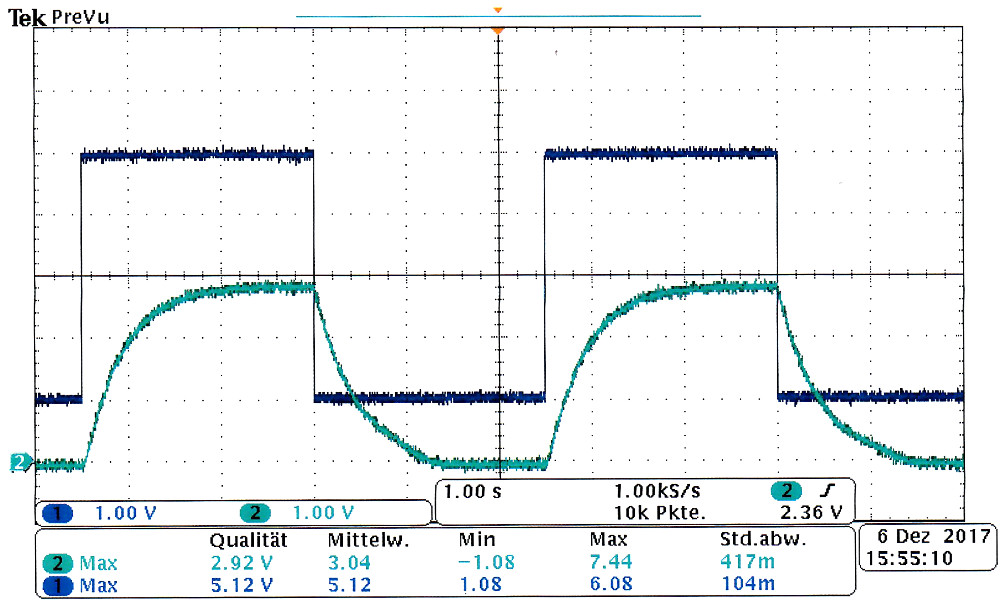
\includegraphics[width=120mm]{jpg/Sinus-KP-klein-KD-gross}
        \end{adjustbox}
        \captionof{figure}{PD-Regelung mit kleinem $K_{\text{P}}$ und großem $K_{\text{D}}$}
        \label{fig:Sinus-KP-klein-KD-gross}
    \end{center}
\endminipage
%
\par
%
\minipage{\linewidth}
    \begin{center}
        \captionsetup{type=figure}
        \begin{adjustbox}{max width=\linewidth, keepaspectratio}
            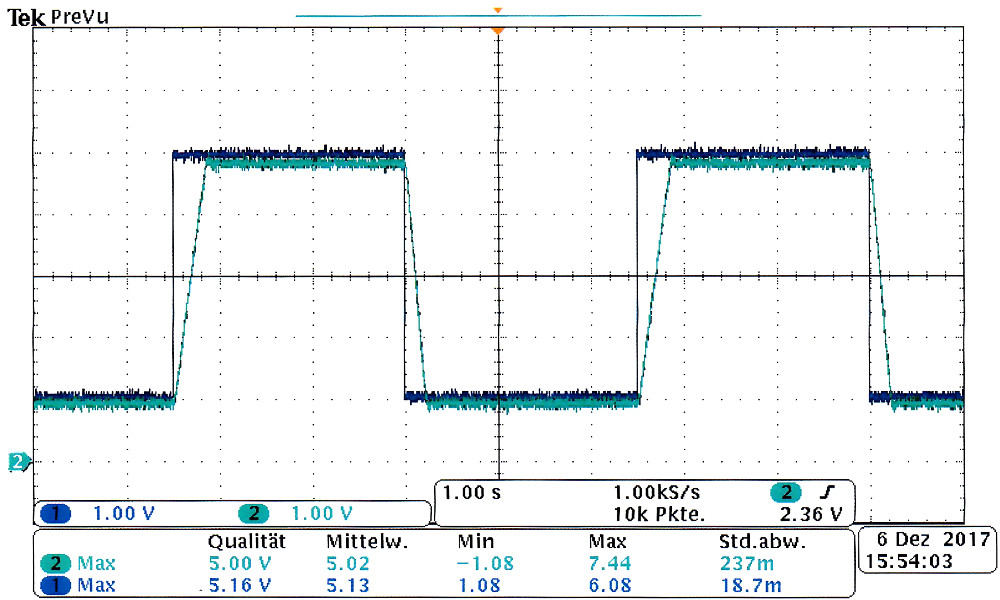
\includegraphics[width=120mm]{jpg/Sinus-KP-gross-KD-gross}
        \end{adjustbox}
        \captionof{figure}{PD-Regelung mit großem $K_{\text{P}}$ und großem $K_{\text{D}}$}
        \label{fig:Sinus-KP-gross-KD-gross}
    \end{center}
\endminipage
%
\par
%
\minipage{\linewidth}
    \begin{center}
        \captionsetup{type=figure}
        \begin{adjustbox}{max width=\linewidth, keepaspectratio}
            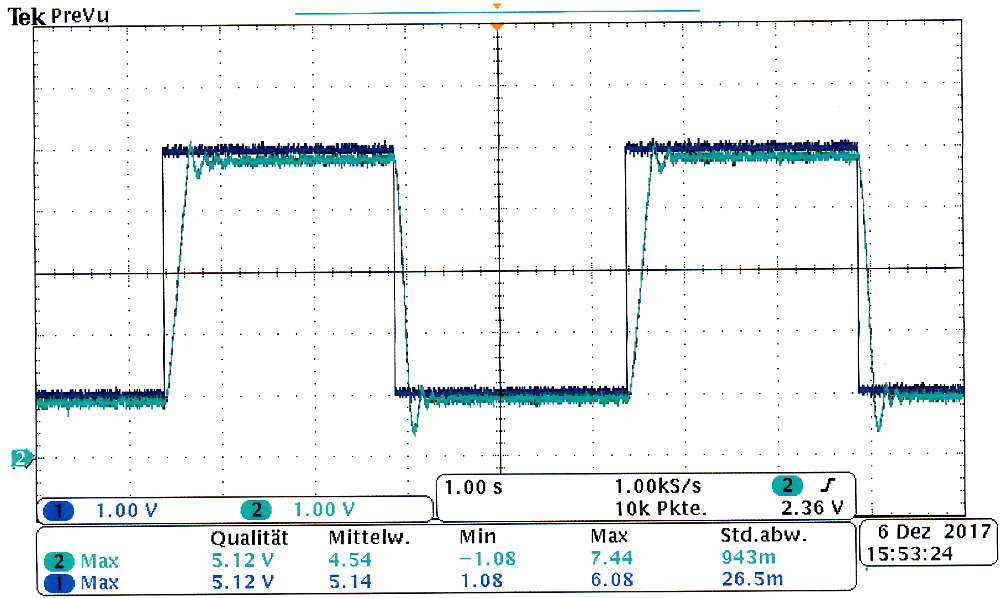
\includegraphics[width=120mm]{jpg/Sinus-KP-gross-KD-klein}
        \end{adjustbox}
        \captionof{figure}{PD-Regelung mit großem $K_{\text{P}}$ und kleinem $K_{\text{D}}$}
        \label{fig:Sinus-KP-gross-KD-klein}
    \end{center}
\endminipage
%
\subsubsection*{Untersuchung PID-Regelung}
%
Nun werden alle drei Regler angeschlossen und man erhält damit eine Kombination aus P-, I- und D-Regler: die sogenannte PID-Regelung.
Wir erreichen ein optimales Ergebnis für großen $K_{\text{P}}$, kleinen $K_{\text{I}}$ und mittleren $K_{\text{D}}$ Parameter.
Die Aufnahme ist in Abbildung \ref{fig:Sinus-KP-gross-KI-klein-KD-mittel} dargestellt.
%
\par
%
\minipage{\linewidth}
    \begin{center}
        \captionsetup{type=figure}
        \begin{adjustbox}{max width=\linewidth, keepaspectratio}
            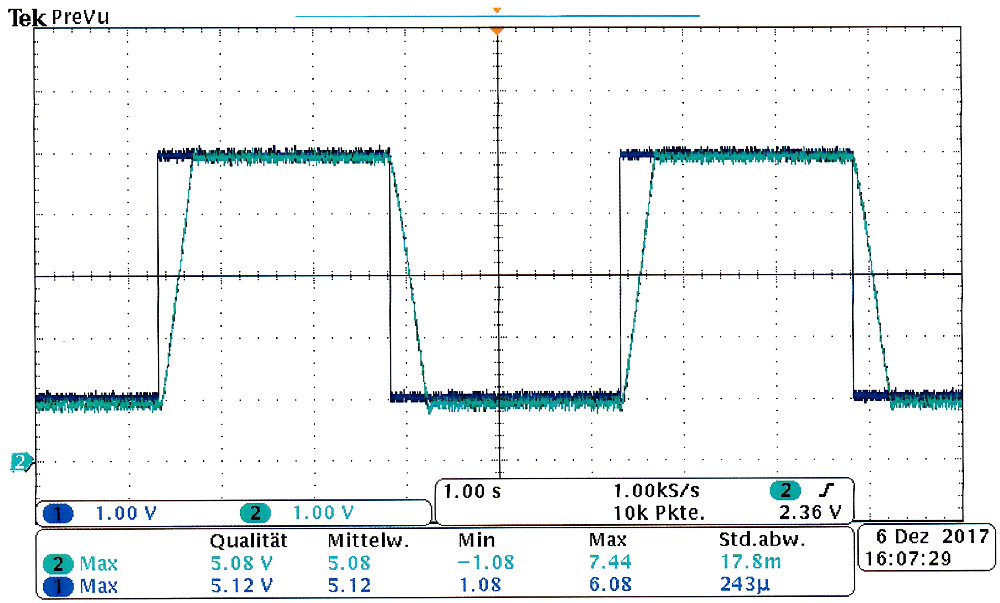
\includegraphics[width=120mm]{jpg/Sinus-KP-gross-KI-klein-KD-mittel}
        \end{adjustbox}
        \captionof{figure}{PID-Regelung mit großem $K_{\text{P}}$, kleinen $K_{\text{I}}$ und mittleren $K_{\text{D}}$}
        \label{fig:Sinus-KP-gross-KI-klein-KD-mittel}
    \end{center}
\endminipage
%
\subsubsection*{Niedrige Motordrehzahlen}
%
Die Sollregelung wird von extern wieder auf intern umgestellt.
Mit dem Sollwert-Potentiometer können wir nun beliebige Änderungen vornehmen und der Istwert folgt dem eingestellten Sollwert ohne Probleme, wie in Abbildung \ref{fig:PID-optimal-Sollwert-manuell} zu sehen.
%
\par
%
Analog dazu ist beim Zuschalten einer Last in Form von Generator mit angeschlossener Glühbirne keine Änderung im Signalverlauf festzustellen.
Der Istwert folgt dem Sollwert konstant.
Mit deaktiviertem Regler sinkt jedoch der Istwert bei zugeschalteter Last auf einen bestimmten Wert ab, bleibt dort konstant und steigt wieder sobald die Last entfernt wird.
Durch den Regler kann der Motor nun auch mit gering gewähltem Sollwert gestartet werden, was ohne Regler nicht möglich war: es musste erst eine bestimmte Schwelle überschritten und dann wieder zurückgestellt werden.
Zudem können generell niedrigere Drehzahlen erreicht werden.
%
\par
%
\minipage{\linewidth}
    \begin{center}
        \captionsetup{type=figure}
        \begin{adjustbox}{max width=\linewidth, keepaspectratio}
            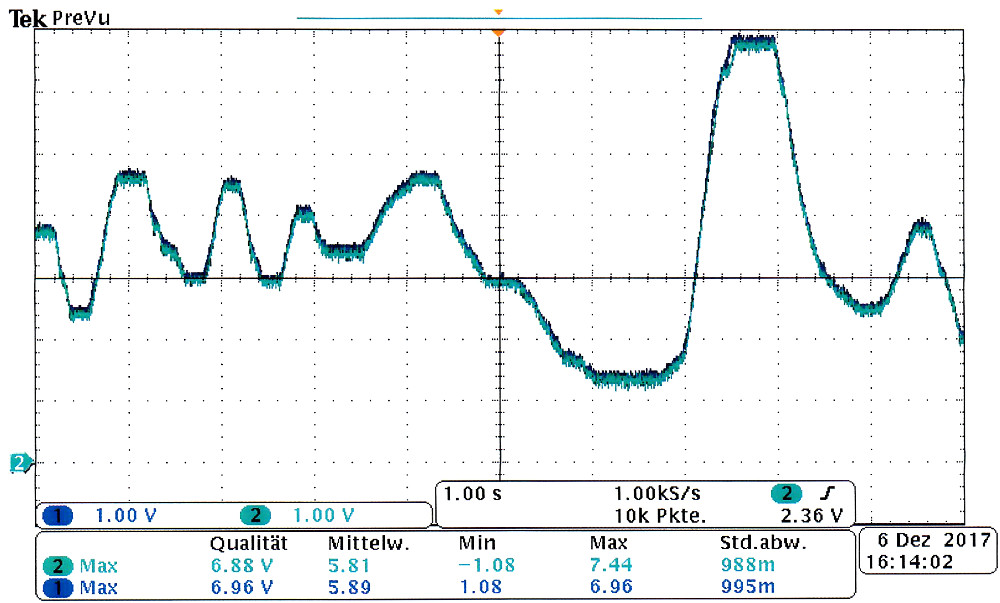
\includegraphics[width=120mm]{jpg/PID-optimal-Sollwert-manuell}
        \end{adjustbox}
        \captionof{figure}{PID-Regelung mit optimaler Kombination aus $K_{\text{P}}$, $K_{\text{I}}$ und $K_{\text{D}}$ bei beispielhafter manueller Sollwert-Regelung}
        \label{fig:PID-optimal-Sollwert-manuell}
    \end{center}
\endminipage
%
\subsubsection*{Andere Signalformen und höhere Frequenzen}
%
Neben dem Sinussignal kann der Regler auch beispielsweise Dreieckssignalen folgen.
Bei höheren Frequenzen lässt die Qualität jedoch nach: bei einem Sinussignal ab etwa \SI{1,5}{\hertz}, bei einem Dreieckssignal ab etwa \SI{0,8}{\hertz}.
Darüber nimmt die Amplitude des Istwert-Signals immer weiter ab und es ergibt sich eine Schwingung um einen konstanten Punkt des Sollwert-Signals.
%
